
\documentclass[twocolumn,10pt]{article}

\usepackage{balance}
\usepackage[margin=1.0in]{geometry}
\usepackage{graphicx}
\usepackage{ifpdf,theorem,tabularx,multirow}

\newcommand{\ie}{{\em i.e.,}~}
\newcommand{\eg}{{\em e.g.,}~}

\begin{document}
\title{Big Data Analysis Exploiting Genome Similarity\\ Qualifying Exam}
\author{Kristal Curtis}
\date{Dec. 13, 2012}
\maketitle

\abstract

As DNA short read sequencing has emerged as an extremely affordable process, efficient and accurate processing of short read data has become the main prerequisite to the use of whole-genome information in a clinical setting.  In this work, we discuss our efforts to improve on the efficiency of current tools, without sacrificing accuracy.  We have mainly focused on identifying and exploiting the similar regions in the human genome, since we have determined that the similar regions serve as the main difficulty in processing short read data.  We have some initial work improving alignment through the use of similar regions, and we discuss our plans to address the rest of the pipeline as well.

\section{Introduction} 

% short read sequencing is becoming cheap; that's exciting because we might be able to use it to study genetic causes of diseases (esp. cancer)
Over the past decade since the Human Genome Project was completed, the cost of sequencing a DNA sample has dramatically declined.  This has been accompanied by an increased interest in studying the molecular causes of diseases, particularly cancer.  In particular, in the case of cancer, the hope is that by identifying genetic drivers of the disease, targeted drugs will be developed to attack these causes rather than indiscriminately attacking many of a patient's healthy cells as well, as is the case with standard chemotherapy.  Many medical practitioners dream of employing whole-genome sequencing as a standard part of caring for cancer patients.

% the data processing is a nontrivial part of the expense, and it'll take over soon since the price of the wetlab portion is falling so steeply
In order for this to become practical, it is necessary for the entire process of sequencing and analyzing a patient's DNA to be cost-effective; the number that is often quoted as the cost target is \$1000.  Currently, the total cost for this process is about \$5000, with \$4000 for the sequencing and \$1000 for the bioinformatics\footnote{These figures are based on a quote received from BGI in early 2012}.  Due to a high degree of parallelism employed by short-read sequencers, the wetlab cost of sequencing a sample is plummeting much faster than Moore's Law.  However, the cost of informatics will decline only as fast as Moore's Law, unless new algorithms are developed.  Therefore, the cost of processing the short read data will soon dominate the cost of sequencing it.

% therefore, we need to work on the processing to make it faster & without trading off accuracy
Therefore, this data processing cost will soon present a major obstacle to clinical adoption of whole-genome sequencing.  In order to realize the dream of including specific information about the genetics of a patient's disease in their course of treatment, we must improve the efficiency of short read processing.  However, we must not trade off accuracy in the process, as accuracy is also an important precondition to the usefulness of this information.

In this work, we discuss our efforts to improve the efficiency, without losing accuracy, of the pipeline to process short read data.  Our efforts have mostly focused on short read \textit{alignment}, which is the first step of the pipeline.  This is a good target for improvement, since it is a very expensive portion of the pipeline.  In addition, since it is the first step of the pipeline, any mistakes incurred at this step will propagate throughout subsequent analysis.  

Through the creation of a new short read alignment algorithm, called SNAP, we have identified that the structure, and specifically the repeat content, of the human reference genome is the main complicating factor in DNA short read analysis.  We will discuss our efforts to identify the DNA repeat content in the human genome in a manner that is driven by the characteristics of the short reads themselves.  We will then present some initial work, as well as vision for further improvement, that exploits the similarity of the genome to improve the efficiency of short read processing.

\section{Background}

In what follows, we provide a review of the literature related to short read alignment, identifying repeat content in the genome, and short read alignment strategies informed by the genome's structure.

\subsection{Improving Alignment with SNAP}
\label{section:SNAP}

My work as part of the SNAP (Scalable Nucleotide Alignment Program) project sets the stage for this work on the importance of similarity and similarity-exploiting algorithms.  SNAP is a fast, accurate short-read alignment algorithm.  Many existing alignment algorithms focus either on speed or accuracy.  SNAP improves on the speed of the so-called fast algorithms while maintaining a high accuracy.

% TODO:  cite BLAST
The original short-read alignment algorithms, such as BLAST, used a hash table to create an index of the reference genome.  Then, given a read to align, they generated a list of candidate locations where the read might match by looking up substrings of the read, termed \textit{seeds}, in the hash table.  To choose a location out of this list, the algorithm would compute the edit distance from the read to the reference at each candidate, and it would report the best of these locations as the alignment for the given read.  Algorithms in this class are generally considered to be accurate but slow.

% TODO:  add citations for Bowtie2, SOAP2
Most of the aligners that are generally considered to be fast are based on the Burrows-Wheeler transform.  These include BWA \cite{Li:2009}, Bowtie2, and SOAP2, among others.  These aligners work by representing the genome as a compressed trie rather than a hash table.  While these aligners are faster than the hash-based aligners, they are less accurate.  They also tend to be more restrictive in the reads that they can align, \ie they permit fewer errors per read, or only errors of a certain type.

SNAP is a hash-based aligner like the first category.  However, it is faster and more accurate than the Burrows-Wheeler aligners.  It achieves this balance by a combination of leveraging resource improvements and algorithmic innovation.  Regarding resource improvements, both DNA short-read sequencers and modern servers have improved.  This results in longer reads, which are easier to align because they permit us to use longer seeds.  Longer seeds are advantageous because they result in fewer matches and therefore fewer locations against which reads must be compared.  Improvements in server architectures mean that it is practical to obtain a server with many tens of gigabytes, or even a few hundred gigabytes, of memory; in fact, servers of this type may be rented for under \$2 per hour via Amazon EC2.  This lets us create a more comprehensive index of the reference genome than was possible when the first hash-based aligners were developed, which has the advantage of resulting in fewer cache misses.

Beyond leveraging improving sequencing and computational resources, SNAP also gains speed by minimizing the number and cost of edit distance checks.  The number of edit distance checks is reduced through the use of long seeds, which have fewer false positive matches in the index.  The cost of edit distance checks is reduced by using the Ukkonen edit distance algorithm, which is less expensive depending on the maximum edit distance permitted.  We leverage this fact by progressively reducing the bound on the edit distance check as we find better and better matches.  We can do this because since the point is to find the best match, as well as to determine whether we can map the read unambiguously, we need only consider the best and second-best matches for the read.  Thus, we need not consider any matches that are worse than the best and second-best we have so far located.  

We have extensively evaluated SNAP on both simulated and real data, as well as both single- and paired-end data.

\subsection{Variant Calling}

The next step after alignment is variant calling.  The goal of variant calling is to identify the locations at which the sample's genome differs from the reference genome, as well as to identify the content of the sample's genome at those locations.  Variant calling usually takes place after the reads have been aligned to the reference genome, via an alignment algorithm like SNAP.  The variant calling pipeline is represented at a high level in Figure \ref{fig:pipeline}.  Variant calling includes locating small variants, called single nucleotide polymorphisms (SNPs), as well as larger ones, called structural variants (SVs).  The most commonly used tool for SNP calling is called the Genome Analysis ToolKit (GATK) \cite{DePristo:2011}.  Several tools for structural variant calling exist.

\begin{figure}
\centering
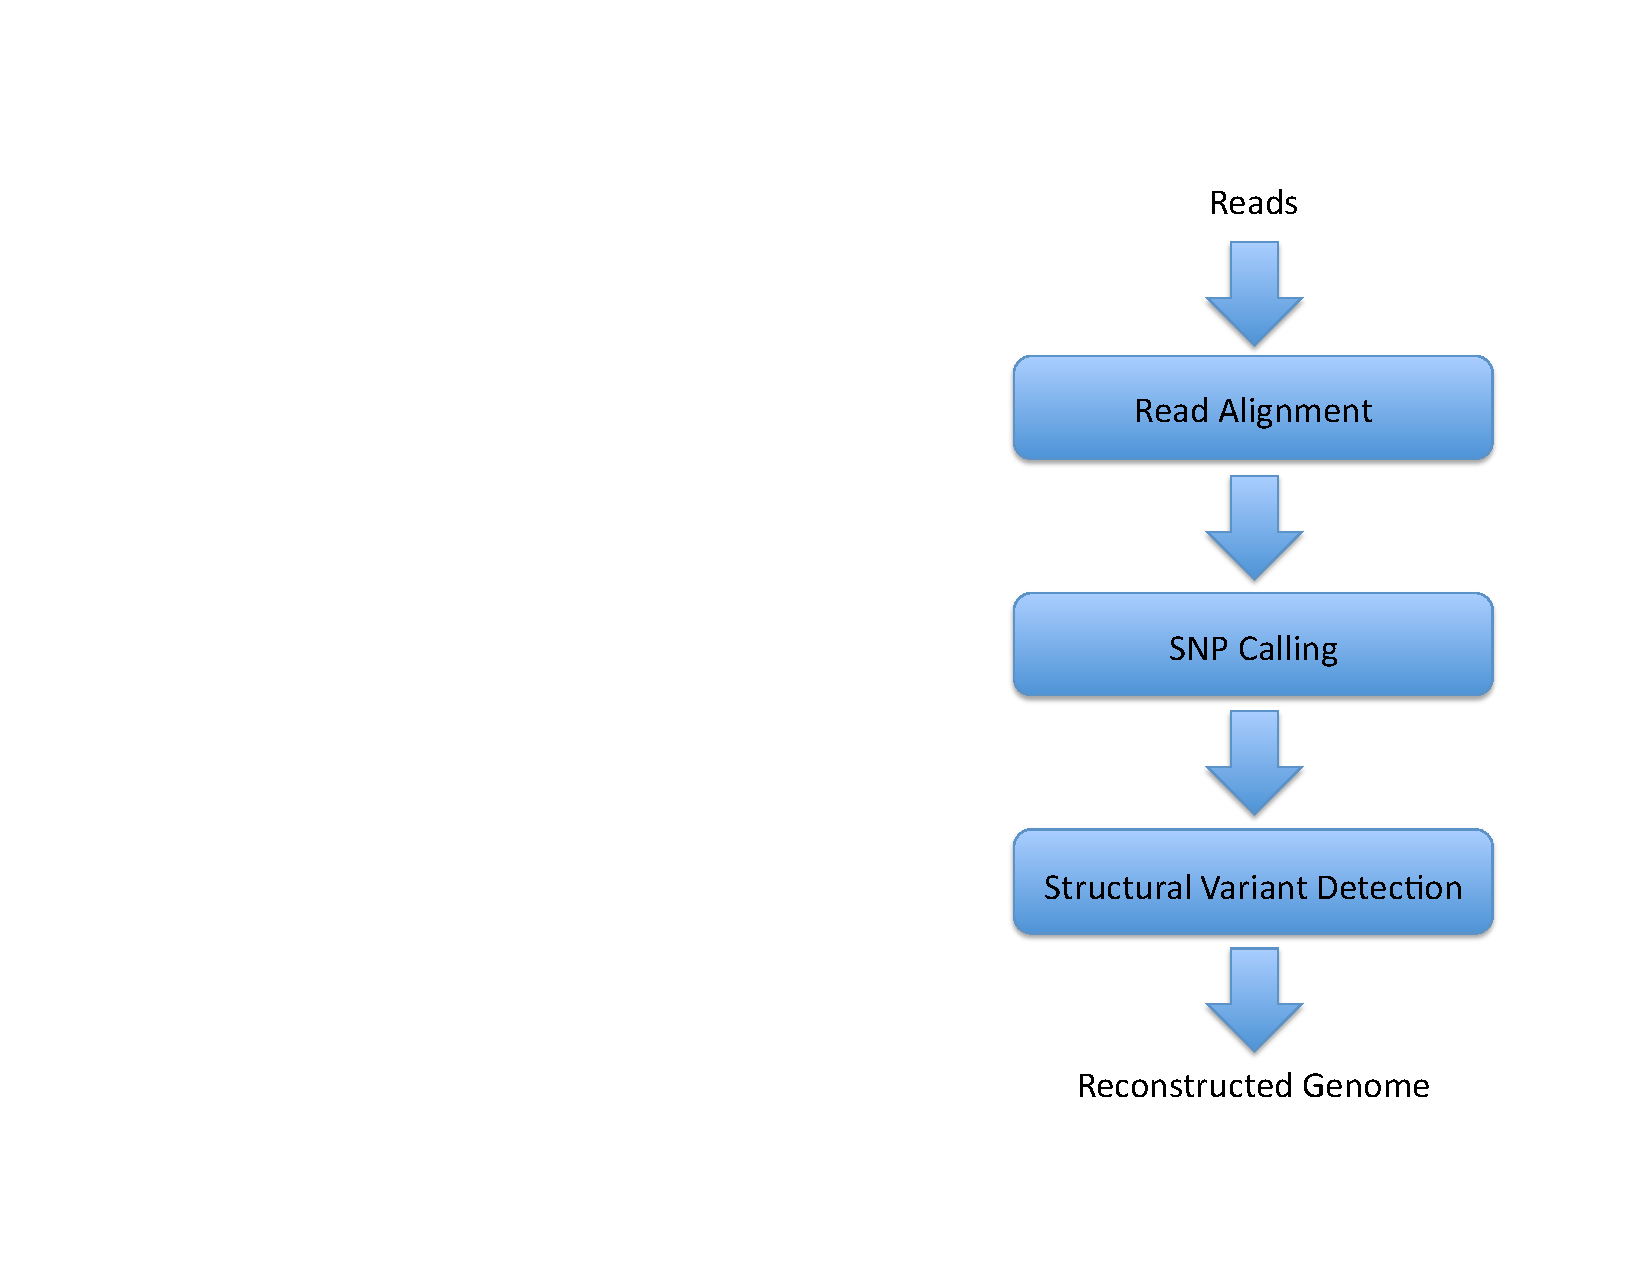
\includegraphics[scale=0.6]{pipeline.pdf}
\caption{Variant calling pipeline, at a high level.}
\label{fig:pipeline}
\end{figure}

The high-level idea of variant calling is to look at all the reads that overlap a particular location and to determine what information those reads collectively contain about the genome content at that location.  This process is illustrated in Figure \ref{fig:variantCalling}.  In the figure, several reads overlap a particular position, and most of them suggest an alternative allele to that possessed by the reference genome (the alternative allele is represented in red).  One of the reads has different content at the given location (represented by a yellow marker); this is likely an error particular to the read, since it appears only in that read.  Thus, the straightforward thing to do at this location is to postulate that the sample's genome has the allele represented by red at that position.

This process is similarly carried out at all locations in the genome.  The output is a list of variants, or positions where the individual's genome differs from the reference genome.  This information is useful for a variety of tasks, such as genome-wide association studies which seek to identify a genetic cause for a particular disease.  

\begin{figure*}
\centering
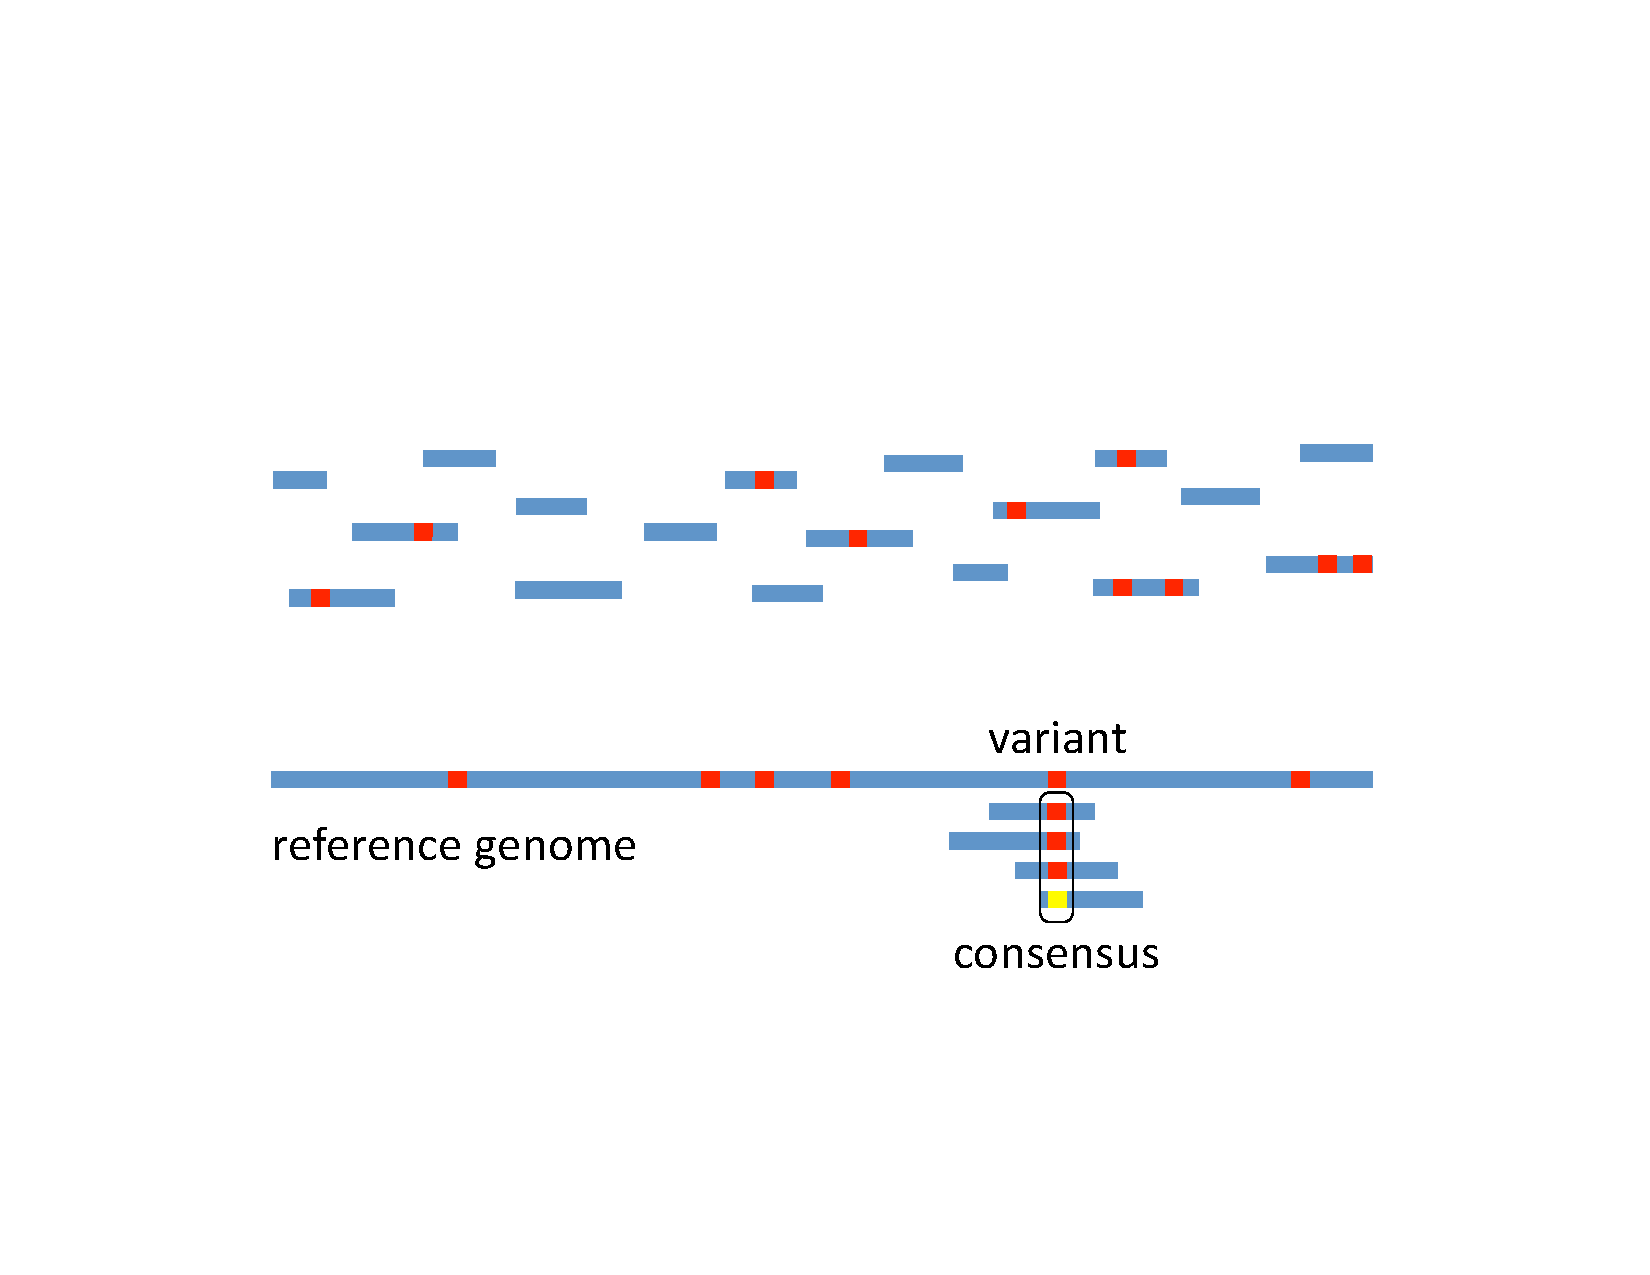
\includegraphics[scale=0.6]{variantCalling.pdf}
\caption{Variant calling overview.}
\label{fig:variantCalling}
\end{figure*}

\subsection{Alignment to Similar Regions}
% based on review paper

An excellent review of how existing short read aligners handle reads that align to many locations is provided in \cite{Treangen:2012}.  It has been established that due to the presence of repetitive DNA, the short read alignment problem is more difficult.  One strategy is to ignore the read, although this can result in a lack of coverage of aligned reads at similar regions in the genome.  Some aligners place the read at its best match, although this can be error-prone.  Some aligners instead choose to report several of the top alignment locations; in the extreme, this strategy can be extended to reporting all alignment locations for a read.  Currently, short read aligners do not identify similar regions in advance and then leverage this information during alignment of potentially ambiguous reads.

\subsection{Clustering the Genome}
\label{section:clusteringTheGenome}

Several algorithms for identifying repeat regions in DNA have been proposed; \eg the Repeat Pattern Toolkit (RPT) \cite{Agarwal:1994}, RepeatFinder \cite{Volfovsky:2001}, RepeatScout \cite{Price:2005}, RECON \cite{Bao:2002}.  In addition, a database called RepBase that contains repeats identified by individual researchers has been compiled \cite{Jurka:2005}.

These repeat identification algorithms all tend to be focused on discovering the repeat structure of a new genome, in hopes of gaining a biological understanding of the origin and function of these repeats.  They tend to be focused on interpretability and therefore favor coalescing repeats into relatively fewer families, since this results in less information to consider.  In addition, they have a very high degree of generality as a goal; that is, they refrain from posing constraints on characteristics such as the size of the repeats.  Instead, they wish to discover repeats of any size, with a high degree of dissimilarity from each other, and even allowing strings of different sizes to be clustered together.  The open-ended nature of the problem that these algorithms are posed to address results in very complicated and computationally expensive algorithms.  While the output may be more suitable for interpretation, it is less usable by algorithms focused on short-read processing.  To our knowledge, there has not been work focusing on finding repeats at the scale of short reads.

\section{The Similarity Problem}
\label{section:similarityProblem}

After implementing the basic SNAP algorithm, we explored how various properties of its search parameters and input data affect its speed and accuracy.  Through this process, we discovered that the main obstacle to both speed and accuracy in alignment is the \textit{similar regions} in the genome.  In what follows, we discuss our observations of how similar regions impact SNAP's performance.  Then, we describe a method for identifying the similar regions, as well as some insights into their characteristics.  We also discuss how we plan to exploit genome similarity throughout the pipeline to improve speed and accuracy of variant calling.

% could also be "Motivation"
\subsection{Observations}

One of our goals following the development of SNAP was to determine the impact of its various parameters on its speed and accuracy.  By accuracy, I mean to encompass both \% aligned and \% error.  Thus, we performed a parameter sweep.  We observed that the only parameter that significantly impacted SNAP's performance was \(h_{max}\), which is the maximum number of genome locations to which a seed could match and still be considered by SNAP.  Seeds occurring at more positions in the genome than \(h_{max}\) are ignored by SNAP, to avoid spending undue time attempting to match reads that are unlikely to be matched uniquely.

Figure \ref{fig:maxHits} shows the results of this parameter sweep.  As we increase \(h_{max}\), the alignment accuracy improves, \ie we are able to align more reads while making fewer errors.  However, this comes at a significant cost to throughput.  The interesting thing about this result is that while you might think that a read that contains popular seeds cannot be uniquely mapped, what we actually observe is that these reads that map to lots of locations actually can be mapped uniquely if we check enough locations, hence the improvement to \% aligned.

\begin{figure*}
\centering
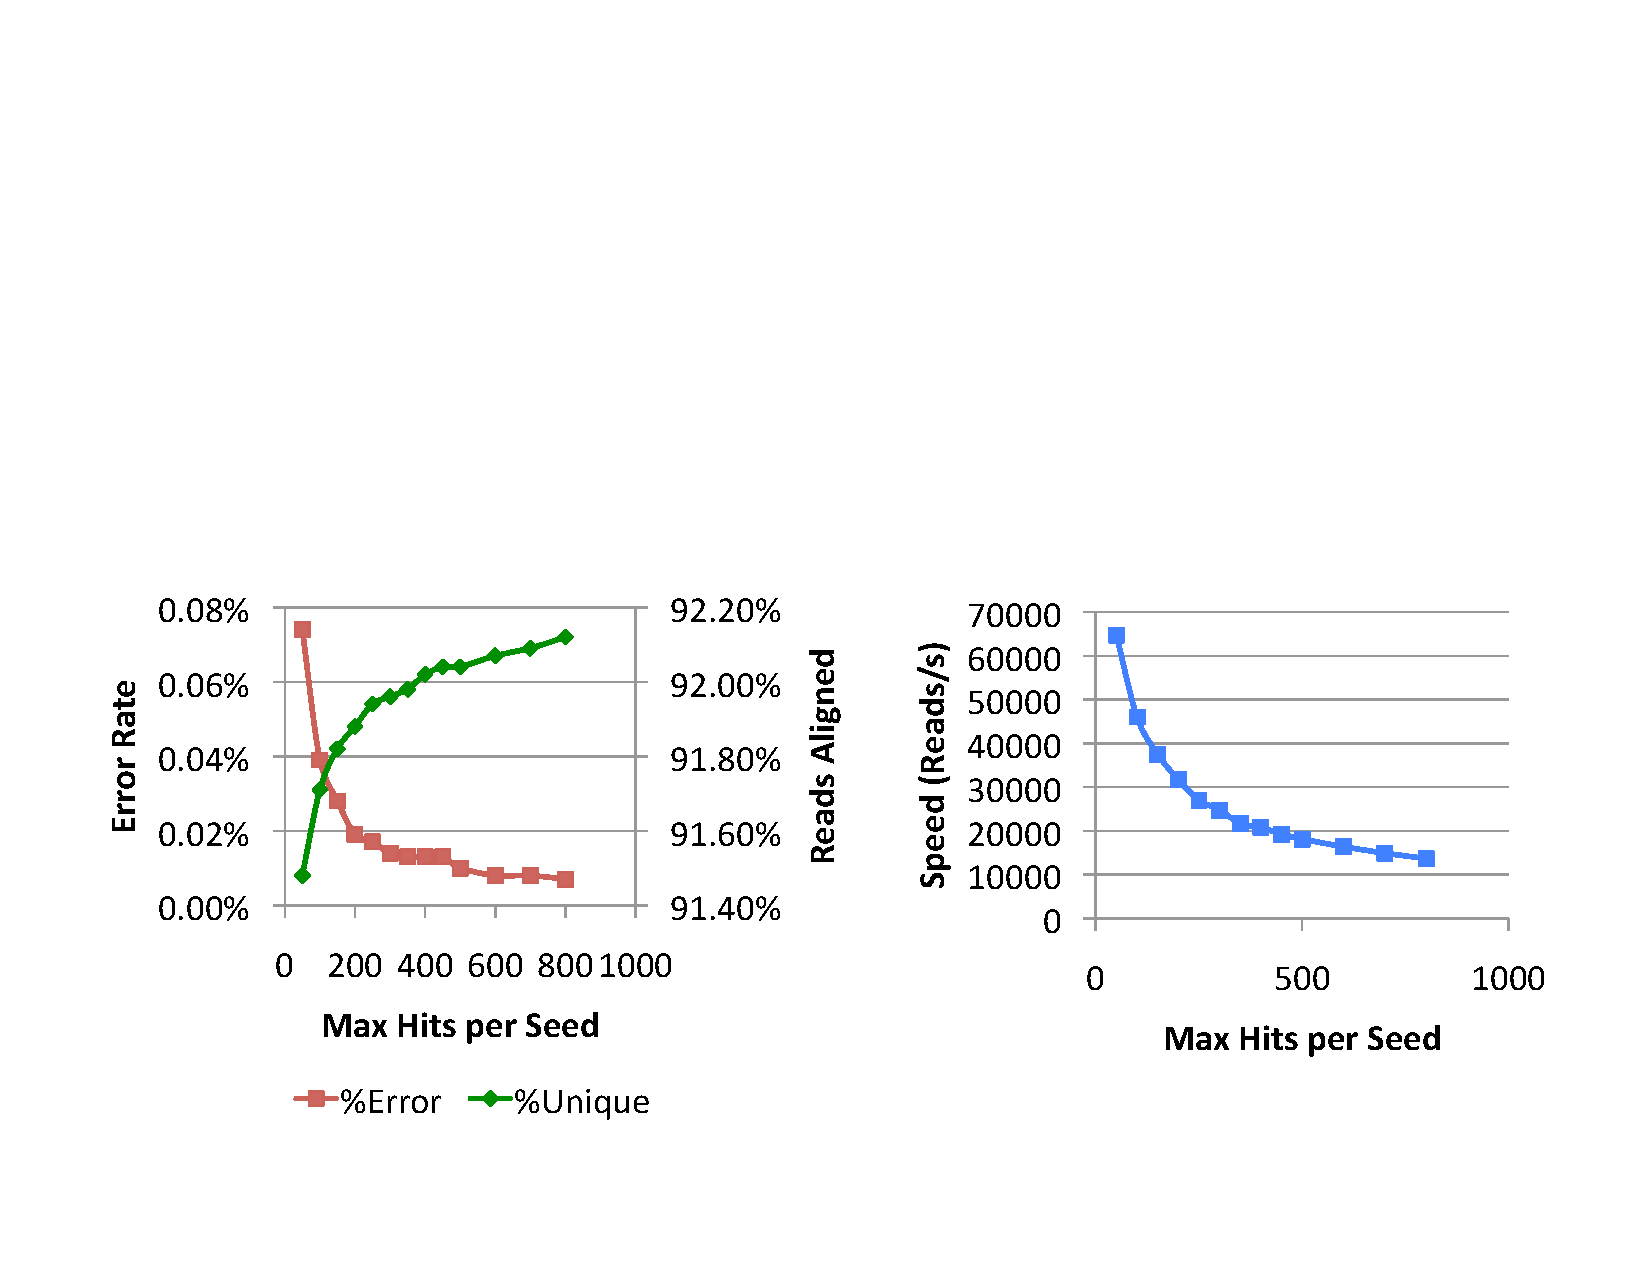
\includegraphics[scale=0.6]{maxHits.pdf}
\caption{Accuracy improves as we increase \(h_{max}\), the number of locations we check per seed, but throughput suffers.}
\label{fig:maxHits}
\end{figure*}

We discovered that this is due to the repetitive nature of the genome.  Exact duplicates are not as confounding, since if the problem were just that there are too many exact duplicates, increasing \(h_{max}\) would not result in any increase in \% aligned, since it would be impossible to find a unique mapping location no matter how many locations SNAP considers.  The difficulty here is caused by near duplicates, which we refer to as \textit{similar regions}.  The presence of near duplicates means that in many cases, it actually is possible to find a unique alignment for a read that contains popular seeds, due to slight differences between the similar regions.  Thus, there is a benefit to checking many locations per read, even though it is expensive.

To confirm our intuition that similar regions are presenting a significant obstacle to alignment performance, we did a simple experiment.  We aligned one million reads, simulated from the whole genome, with SNAP.  Then, for the reads which SNAP aligned incorrectly, we checked whether the read belonged to a cluster.  How the clusters were located will be described in Section \ref{section:identifyingSimilarRegions}.  Our findings were surprising; out of the 227 errors that SNAP made, 195 (86\%) were in clusters.  For reference, only 8\% of the positions in hg19 belong to a cluster.  Therefore, the clusters, though making up a small fraction of the genome, make a huge impact on alignment performance.  Thus, it is essential to improve the handling of these reads in order to improve alignment performance.

\begin{figure*}
\centering
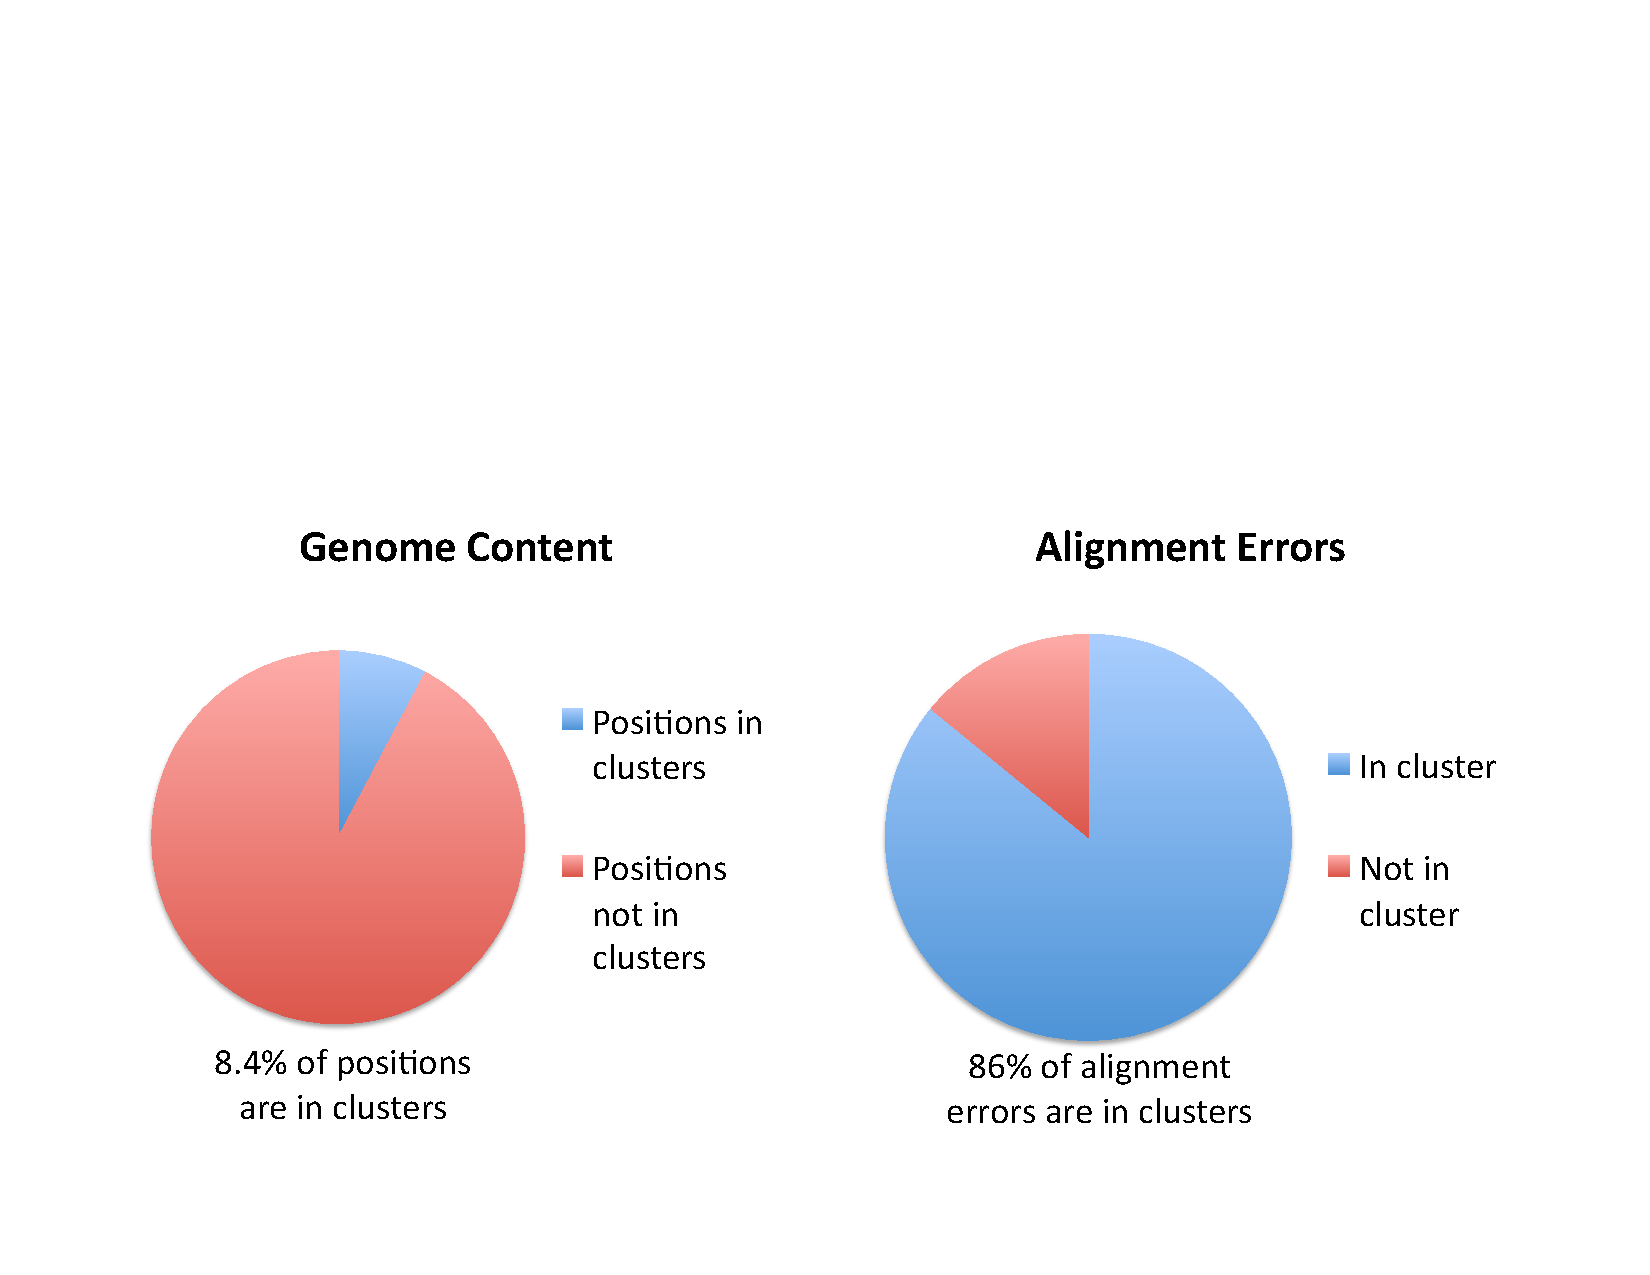
\includegraphics[scale=0.6]{errorsInClusters.pdf}
\caption{Despite the fact that a small fraction of the genome belongs to a cluster, a significant fraction of alignment errors occur in clusters.}
\label{fig:errorsInClusters}
\end{figure*}

\subsection{Identifying Similar Regions}
\label{section:identifyingSimilarRegions}

% talk about how union find works
% TODO:  want to mention that this is with Hamming distance rather than full edit distance?
The straightforward approach to find clusters would be to create a graph where the nodes are the substrings in the genome and there is an edge between any two nodes that are sufficiently similar.  Then, the clusters correspond to the connected components of this graph.  However, since there are over 3 billion substrings of length 100, the length of the short reads we are using, both building this graph and then the subsequent step to find the connected components are very expensive.  Therefore, we chose to approximate this approach by using the well-known \textit{union-find algorithm}.  In union-find, each substring starts in its own cluster.  Then, whenever two substrings are sufficiently similar, we merge the two clusters.  The output of this process is similar to the connected components of the graph identified by the straightforward approach; however, the union-find implementation is much more efficient.  In order to determine which clusters to merge, we use the SNAP index to find all locations to which a substring's seeds map.  Thus, we avoid doing the full \(N \times N\) comparison of all the substrings in the genome.

% talk about how I used Spark for the implementation
Though the union-find algorithm is more efficient than the na\"{\i}ve connected components approach, it is non-trivial to implement it so that it will run in a practical amount of time on the whole genome.  From the initial version that ran on chromosome 22 to the current version that runs on the full hg19, several implementation changes were needed.  The main change was going from a serial implementation to a parallel version using Spark \cite{Zaharia:2012}.  The parallel version finds clusters in each partition, and then it merges the clusters to produce clusters that are present in the genome overall (Figure \ref{fig:sparkUnionFind}).  Once we had a parallel implementation, we had to do several tricks to make it scale, such as changing the partitioning scheme, using a feature of Spark called accumulators to avoid storing intermediate results, and changing the representation of genome locations so that they could be stored in 4-byte integers instead of 8-byte longs.  These changes were mainly motivated by saving memory.

\begin{figure*}
\centering
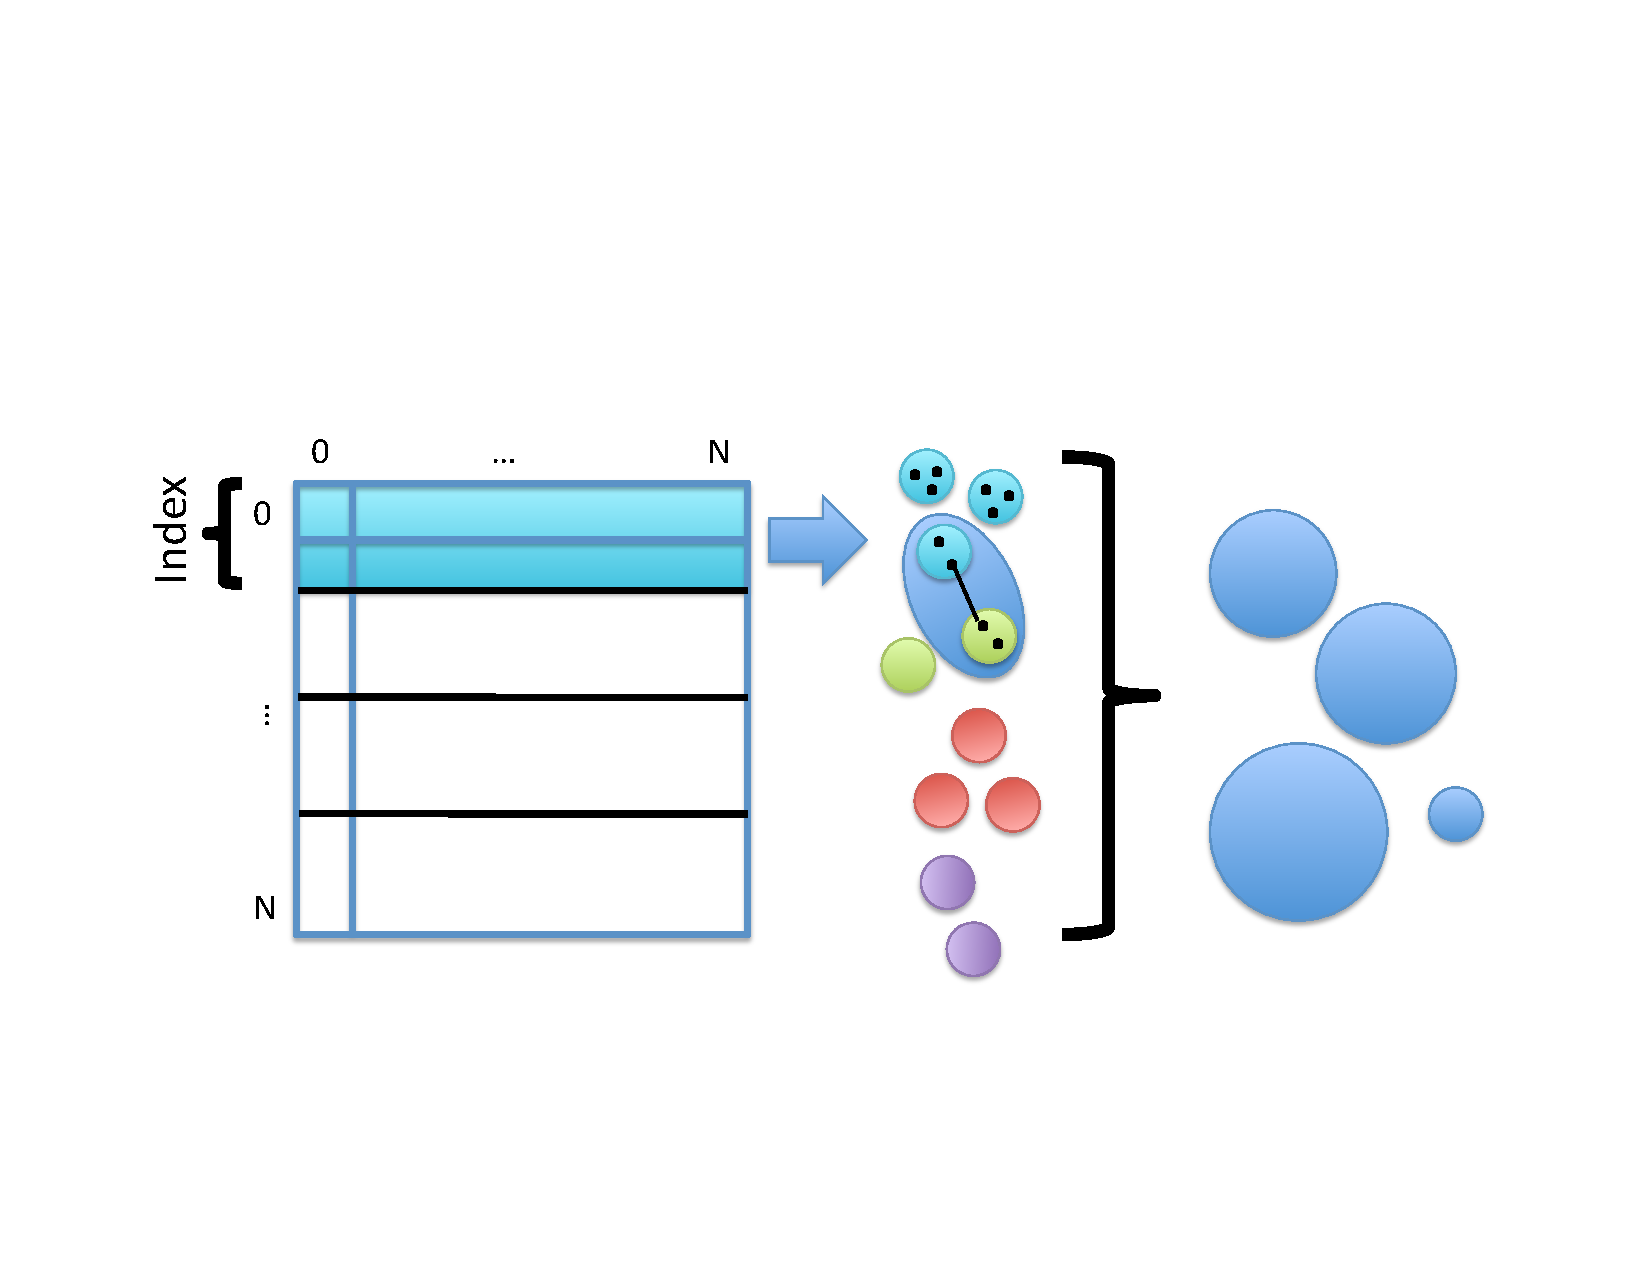
\includegraphics[scale=0.6]{sparkUnionFind.pdf}
\caption{Union-find implementation via Spark.  Parallel implementation involves partitioning the genome.  We find clusters in each partition separately and then merge them to obtain clusters in the genome overall.}
\label{fig:sparkUnionFind}
\end{figure*}

% talk about the pros/cons of this approach
Compared to other approaches to clustering the genome (see Section \ref{section:clusteringTheGenome}), our approach has several advantages.  First, because our approach is driven by the characteristics of the short reads themselves, rather than being motivated by a more biological desire to better understand the repeat characteristics of the genome, our problem is more constrained.  Many of the previous approaches to clustering the genome attempt full generality, without imposing any constraints on repeat length, and allowing many only marginally related substrings to belong to the same repeat family in the interest of reducing the number of repeat families to enhance interpretability.  However, this results not only in algorithms that are very complicated and computationally expensive but also in output that is difficult to utilize for short-read processing.  Our more constrained problem, where we fix the length of any substrings considered to be the same as that of the short reads, is simpler to tackle and is therefore more amenable to an efficient algorithm.  
% still need to talk about cons

The downside to our approach is that since our setting is completely unsupervised, the clusters are difficult to evaluate via an intrinsic metric (\ie one focused solely on the clusters rather than on how the clusters benefit an application in which they are used).  In the situation where labeled data exists (\eg \cite{Cohen:2005}), various metrics such as cluster purity that give a sense for how cohesive the clusters are may be used.  However, in our setting, we lack labeled data.  Some of the previous work attempted to get around this issue by comparing to the data in RepBase.  % TODO:  need citation to RepBase here
However, this comparison is harder in our case, due to the different constraints of our problem.  Therefore, we rely mostly on extrinsic evaluation criteria -- \ie, whether our clusters improve the performance of short read analysis.

% talk about the results
We used a merge distance of 4 based on our experiments with varying the merge distance and looking at the results on single chromosomes.  With smaller distances, the clusters turn out to be too small to make much impact.  With larger distances, the downstream performance degrades too much because the clusters get too bloated.  However, this choice of merge distance is impacted by the extrinsic criteria that are identified, which we will discuss in more detail in Section \ref{section:exploitingSimilarityInAlignment}.  The similar region finder tool applied to hg19 took 126 hours on a single node with 16 cores, or about 2016 CPU-hours.  While this took a few days, it is important to note that the results could be obtained faster by scaling out onto multiple nodes with just a change to the job configuration since we used Spark.  The tool used about 100 GB of memory, which is practical on modern servers.  The output size is 2.8 GB, with 39,992,540 clusters, where a cluster is defined as having at least two members.  The number of genome positions in these clusters is 263,230,347, or 8.4\% of the 3.1B positions in hg19.

\section{Vision for Exploiting Similar Regions}
\label{section:visionExploitingSimilarRegions}

In Section \ref{section:similarityProblem}, we discussed how genome similarity makes short-read processing, specifically alignment, more challenging, and we presented a method for locating the similar regions in the genome.  In this section, we will discuss how to exploit the similar regions that we have identified to improve short-read analysis.  We will begin by describing ongoing work that aims to improve alignment performance by using similar regions.  We will also discuss plans for future work in which we will make use of the information about similar regions in subsequent stages of the pipeline.

\subsection{Exploiting Similarity in Alignment}
\label{section:exploitingSimilarityInAlignment}

% most straightforward:  use clusters in the best-matcher
The most straightforward way to utilize the clusters we produced is to augment SNAP so that it uses information about whether a particular genome position belongs to a cluster.  In the regular version of SNAP described in Section \ref{section:SNAP}, alignment errors are usually due to the situation illustrated in Figure \ref{fig:simAwareSNAP}(a).  Due to the setting of \(h_{max}\), SNAP may consider only some of a read's candidate locations.  This leads to alignment errors when SNAP chooses a location out of the ones it has considered, while the correct location was skipped.

Our idea is to extend SNAP to be aware if a read's candidate locations are in a cluster.  This idea is illustrated in Figure \ref{fig:simAwareSNAP}(b).  Instead of considering each location on its own, without regard to its cluster status, we check for each of a read's candidate locations whether that location belongs to a cluster.  If it does, we automatically pull in all the members of the cluster and compare the read to each of them.  This helps us avoid missing good locations where our read might align (due to \(h_{max}\) being set too low).

\begin{figure*}
\centering
\begin{tabular}{c c}
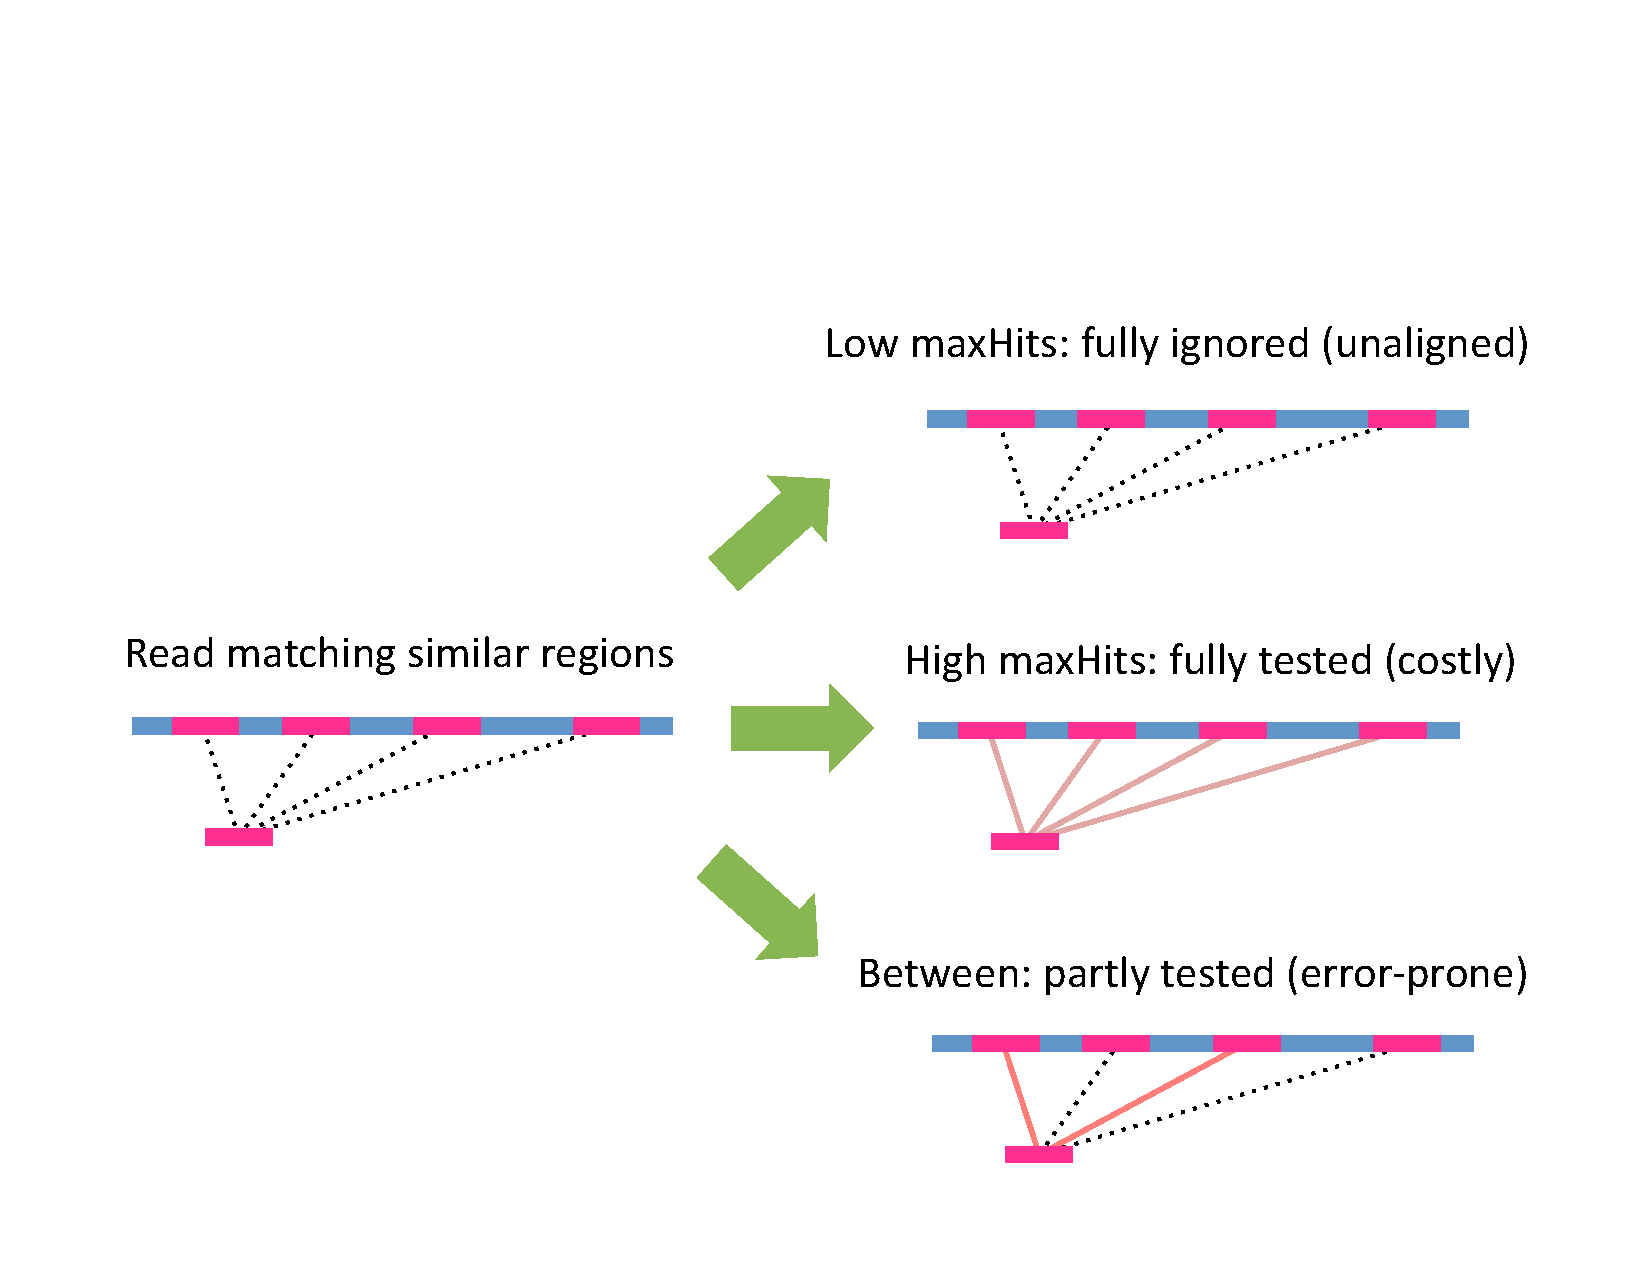
\includegraphics[scale=0.33]{snapWithoutClusters.pdf} & 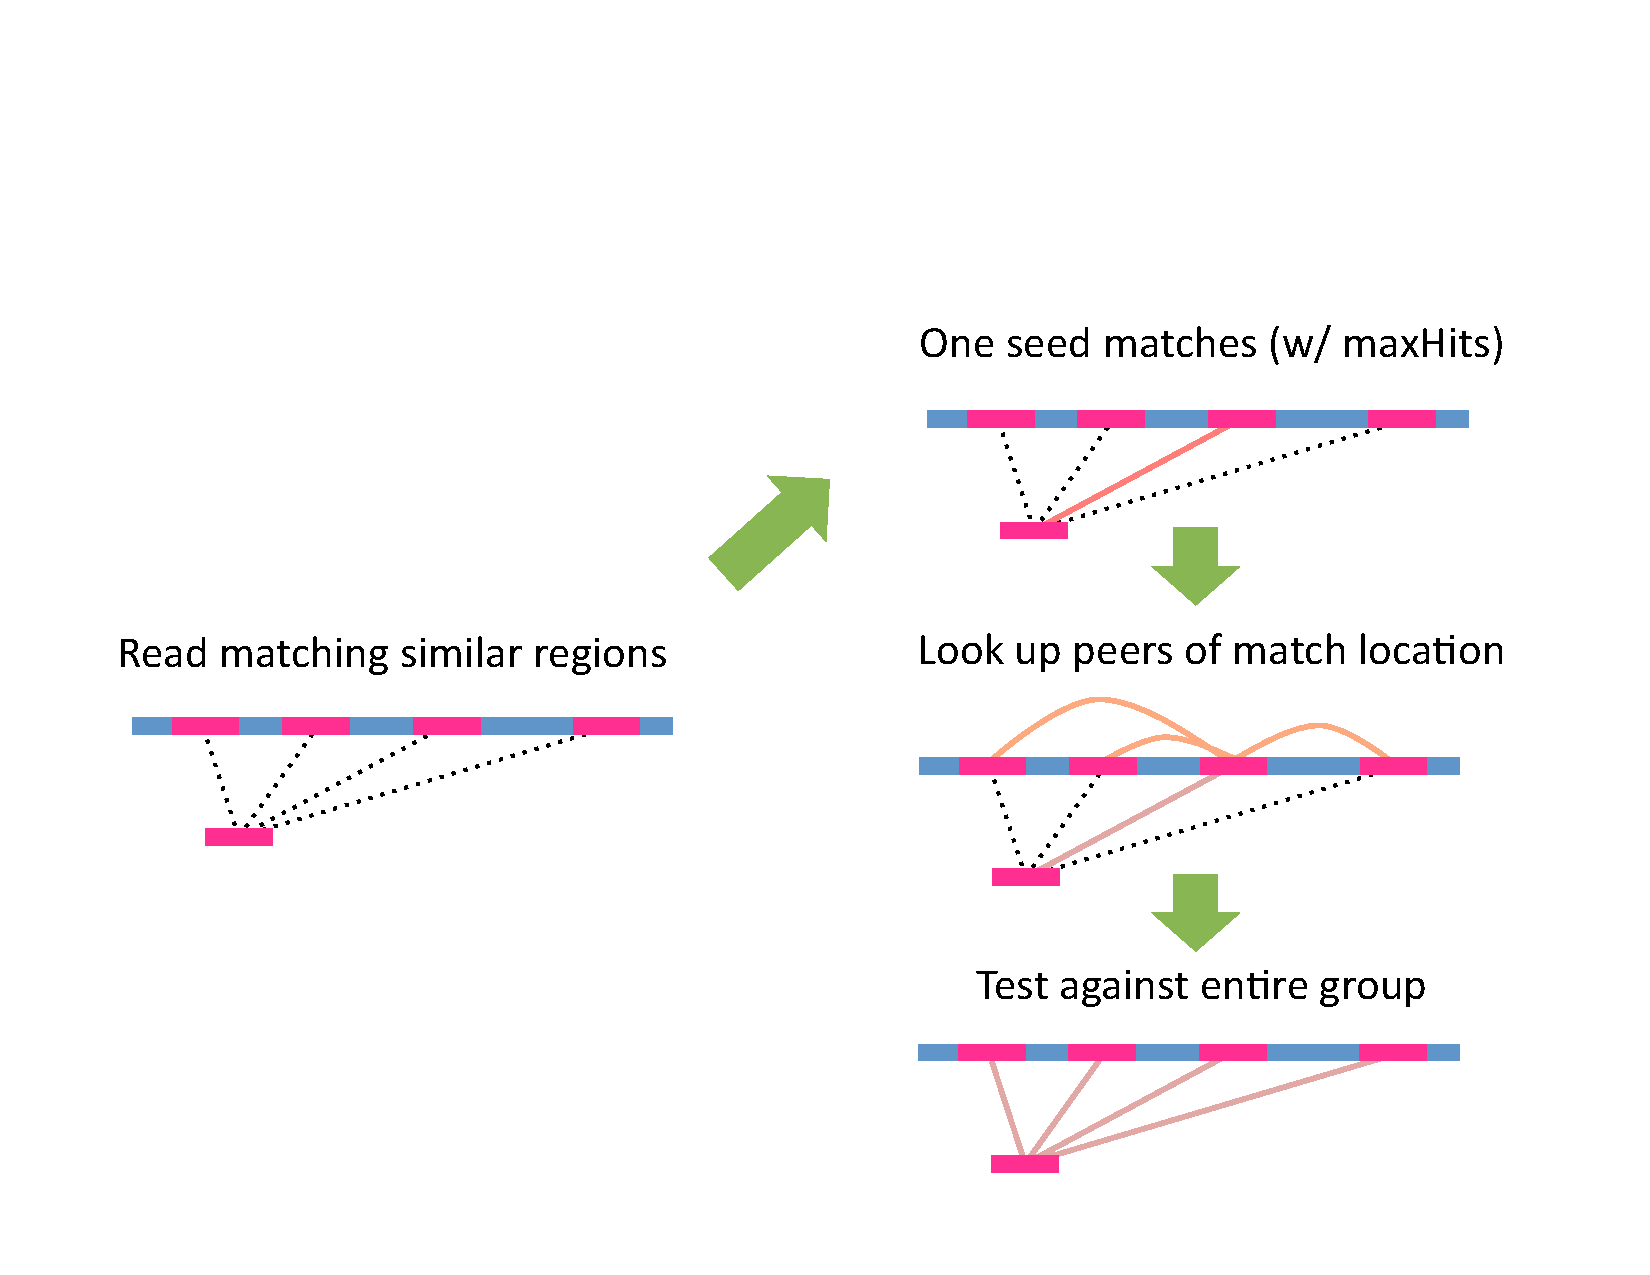
\includegraphics[scale=0.33]{simAwareSNAP.pdf}\\
(a) & (b)\\
\end{tabular}
\caption{SNAP, with and without clusters.  (a)  Without clusters, SNAP may miss some good locations for a read, causing errors.  (b)  With clusters, when SNAP finds that a read matches well against a particular location, it also checks the peers (\ie cluster members) of that location.  This avoids missing locations to which the read may align better than the given location and cuts down on the error rate.}
\label{fig:simAwareSNAP}
\end{figure*}

% say this will improve accuracy, b/c you're comparing against more locations, but you want to do this without losing too much speed
This approach is bound to improve alignment accuracy, since the effect of the clusters is that you compare against more locations and are therefore more likely to find the best location to which the read aligns.  The main challenge, then, is to perform this similarity-aware alignment efficiently.  

% discuss some of the techniques we're using
Presently, we use three techniques to improve the similarity-aware SNAP's performance.  First, we create a special index that is informed by the cluster membership of the genome positions.  In the normal SNAP index, we insert into the hash table a given seed and the position(s) at which it may be found in the genome.  In our similarity-aware index, we modify this approach, in that if a seed found at a given position is in a cluster, instead of storing that position with the seed in the index, we store the cluster ID, which we define to be the first (\ie with the lowest index) member of the cluster.  This avoids an extra step of determining, once you know that a position is in a cluster, which cluster to which a position belongs.

A second technique we use to reduce alignment latency is intra-cluster pruning.  The idea here is that we want to be able to tolerate clusters that may be a little too inclusive, since clusters with more members result in higher accuracy (as more locations are being checked), and because as mentioned in Section \ref{section:identifyingSimilarRegions}, tuning the clusters from our union-find approach is not straightforward.  Therefore, we introduce a preprocessing step in which for each cluster, we determine the consensus string (by simply taking the most popular base at each position), as well as each member's differences from the consensus.  Then, when we decide we want to compare a read to a particular cluster, we use the triangle inequality to filter out members that we know are too distant from the read.  

Third, we have developed a version of the edit distance algorithm that exploits the similarity among the cluster's members.  The idea here is that the strings in a cluster are all very similar to each other, so it is wasteful to compare the read separately against all the locations.  Instead, we compare only against the differences between each cluster member and the consensus string.

% this might be a good place for DP & AF's "hypothetical" graph

% talk about future work to improve the speed further
% discuss how we've done profiling and we need to optimize the indexing scheme, given the memory access patterns we've observed

% extension:  use them in the all-matcher
Another application of the clusters related to alignment is creating an \textit{all matcher} version of SNAP, where instead of returning the single best location where a read matches (or no location, if no confident alignment is available), we return all locations to which SNAP matches within a given edit distance.  All matchers tools are useful for several reasons.  First, some of the structural variant detection tools (\eg VariationHunter) rely on such information \cite{Hormozdiari:2009}.  Current all matchers, such as mrFAST \cite{Alkan:2009}, are painfully slow.  % TODO:  give some #s here
Therefore, creating a faster version of an all-match aligner would make it easier and more practical to use tools like VariationHunter.
We provide the performance results of our all-matcher in Table \ref{table:allMatcher}.  Through the use of some of the techniques presented in the context of the best-match version of SNAP (see Section \ref{section:exploitingSimilarityInAlignment}), we are able to achieve a speedup over the regular SNAP all-matcher.

% give the results we have for the all-matcher (just for chr1-3)
\begin{table*}
\centering
\begin{tabular}{| l || c | c |}
\hline
\vrule height 10pt depth 0pt width 0pt \textbf{Algorithm} & \textbf{Reads/s} & \textbf{Speedup}\\
\hline
\vrule height 10pt depth 0pt width 0pt Regular SNAP & 2125 & -\\
\hline
\vrule height 10pt depth 0pt width 0pt Sim-aware SNAP, regular index & 2358 & 1.11\\
\hline
\vrule height 10pt depth 0pt width 0pt Sim-aware SNAP, sim-aware index & 2920 & 1.37\\
\hline
\end{tabular}
\caption{Using clusters in the all matcher version of SNAP results in a speedup over the regular SNAP all-matcher without clusters.  Results shown were obtained aligning one million simulated reads from chromosomes 1-3.}
\label{table:allMatcher}
\end{table*}
% TODO:  add a line in the table for mrFAST, and maybe mrsFAST as well?

% talk about how we're still working on improving the results
With both the best-match and all-match versions of SNAP, we have spent some time doing profiling to determine how to further improve the speedup obtained by using the clusters.  Our main insight is that the similarity-aware versions of SNAP spend a lot more time in cache misses, each of which costs hundreds of CPU cycles, than the regular version of SNAP.  These cache misses result when the similarity-aware SNAP queries the similarity map to determine whether a given position is in a cluster because the similarity map is too large to fit in the cache.  Therefore, we are currently devising a strategy to alter the similarity map representation so that it will fit into the L3 cache; we are aiming to make it fit in 8 MB.  We plan to use Bloom filters to represent the positions, so that we will need only 5 bits per position.  We also plan to store only the cluster IDs in the similarity map, rather than all the positions that are in clusters.  We expect that this will enable us to further improve the speedup obtained.  However, given that SNAP's memory access patterns have been heavily optimized, the fact that the less mature versions of our similarity-aware best- and all-match algorithms are near or slightly outperforming the standard SNAP is encouraging.  %  TODO:  is this true?

% this part is important!
\subsection{Exploiting Similarity throughout the Pipeline}

Having observing the impact of genome similarity on alignment, and having demonstrated that exploiting similarity will enable us to improve on alignment, we now look to the rest of the pipeline with an aim to improve downstream processing as well.  As before, we are interested in improving on both the speed and accuracy of current tools.  In what follows, we discuss our plans for utilizing similarity information throughout the pipeline.

\subsubsection{Mapping Quality}

One important direction for improving the stages that are downstream from alignment is producing mapping quality (MAPQ) values.  Currently, SNAP lacks the ability to report a broad spectrum of MAPQ values.  Instead, it basically employs a binary strategy:  if SNAP is confident about the alignment (\ie believes the read to be uniquely alignable), it reports a MAPQ of 60; otherwise, if it believes that the read can only be aligned ambiguously, it reports 0.  Therefore, an obvious extension to SNAP would be reporting mapping quality values that span the full range rather than just giving a binary response.  This would be useful because even in the case where SNAP believes that it has found an unambiguous best match, downstream stages would benefit from knowing how confident SNAP is about that value.

Mapping quality was introduced in the context of the MAQ aligner \cite{Li:2008}.  It was extended to allow SNPs and indels in the context of Stampy \cite{Lunter:2011}.  The goal of a mapping quality score is to provide the probability that the read has been misaligned.  To do this in full, it is necessary to compare how well the read aligns at the chosen location to how well it aligns at every other location in the genome.  Obviously, this is prohibitively expensive.  Therefore, this quantity is approximated, generally by considering the best and second-best hits.  The MAQ mapping quality formula considers the base quality values at read positions that do not match the reference at the best and second-best matching genome locations.  They also consider the number of hits with the same number of mismatching bases as the second-best hit.  The idea, then, is that if a read has many locations that are almost as good as the best one, you will be less confident about aligning it.

While a potentially valuable signal to downstream analysis, MAPQ values are generally regarded to be unreliable.  However, downstream analysis does rely on these values, \eg by only considering reads that have been mapped with a MAPQ above a certain threshold.  This results in loss of data that could potentially be useful.  One step that pipelines take to deal with this issue is quality score recalibration \cite{DePristo:2011}; however, this process is very expensive and also potentially error-prone.  Therefore, an improvement to MAPQ would not only be an improvement to SNAP, but it would also potentially improve the speed, by avoiding recalibration, and accuracy, by providing better information about which reads to trust, of the later stages of the pipeline.

Our idea is to not only add the existing approach to MAPQ to SNAP, but also to improve on MAPQ using our similarity information.  We plan to follow the existing approach that takes into account other locations that are candidates for where a read may match.  The clusters will provide a useful signal to where else the read may match, while still maintaining an efficient MAPQ computation.  The idea is that if a read is aligned to a cluster, you automatically know many other locations where it will likely align well.  Therefore, you can take this information into account when you compute the MAPQ score.  The hope is that using clusters, you will get more of the potential matches for the read than you would otherwise, and therefore your approximation should be better than it would be if you missed some of these potential matches.  Recall that the ideal scenario would be comparing against all other locations in the genome; while this is intractable, we can further approach this ideal by using the cluster information.  Recall also that the great majority of alignment errors occur in clusters.  Therefore, just the fact that a read aligns to a cluster location is a powerful signal that the alignment may be incorrect.
% this paragraph probably needs work!  maybe talk about the likelihood that errors are in clusters first, then the advantage of getting more positions to compare against

% pipeline -- use it as a signal to where to spend extra processing time (eg, ravi's SV)
\subsubsection{Variant Calling}

% say something about existing variant calling approaches
Another area where we believe we can exploit the similarity in the genome is in variant calling.  Existing variant calling pipelines such as the GATK \cite{DePristo:2011} are very computationally expensive.  They are also very complicated, not only to run but also to understand what each stage is doing, much less to get a sense for the value that each stage contributes to the final outcome.  Thus, practitioners usually treat them as a black box, without getting much insight into the results that are produced, but rather being required to accept them without question.

% talk about how we want to do things differently:  do something simple/naive on the easy regions; do more on the harder regions
Our goal is to produce a pipeline that is not only more efficient than existing approaches, but also simpler to understand and to use.  We also aim to improve on the accuracy of existing tools.  Our main strategy is, for each region of the genome, to classify the region as either easy or hard, and then to either utilize a na\"{\i}ve variant caller or a sophisticated variant caller, respectively.  We believe that this strategy will allow substantial computational savings, since it is likely that a small fraction of regions fall into the hard category.  Therefore, we will be able to use the simple variant caller most of the time.

% talk about how we'll use clusters as a signal for where the harder regions are
One of the ways that we plan to utilize similarity to improve variant calling is by using the clusters as one of the signals for where the hard regions are.  Since we have already observed that alignment errors are highly concentrated in similar regions (Figure \ref{fig:errorsInClusters}), we believe that these alignment errors will also have a negative impact on our variant calling in these regions.  Therefore, a first step to this process will be to automatically consider any region that falls within a cluster as a hard region, and consequently to devote more processing there.

% might want to jointly consider clusters since reads may be aligned among different cluster members
One idea we have for what kind of sophisticated processing might be necessary in these hard regions, identified as such because of their cluster membership, is to jointly consider regions that co-occur in a cluster.  This is motivated by the fact that since alignment errors occur predominantly in clusters, reads are likely to be somewhat scattered among different cluster members.  Therefore, we could possibly improve performance in these regions by utilizing the knowledge that reads that belong to a particular region may have been assigned elsewhere.  This sort of joint consideration should allow us to disentangle these reads and reassign these reads to their correct location.  We hope that this will lead to an improvement in variant calling accuracy in these regions.

% might want to use this with all-matcher -- let reads align to multiple places, then jointly consider those regions to figure out where the reads probably came from
Another possibility is to use this in conjunction with the all-match version of the aligner.  In this situation, rather than forcing reads that align to clusters to align to a single best location, which may or may not be correct, we would allow these reads to align to many or all of their suitable locations.  Then, these reads could contribute to variant calling at multiple locations, which we would consider jointly.

\section{Research Timeline}

% Paragraph on finishing the SNAP paper with cluster-informed MAPQ
\subsection*{Spring 2013}
I plan to focus on implementing an expanded version of MAPQ, informed by clusters.  This will provide an important yet currently missing feature of SNAP.  Given this feature, we will submit a SNAP paper.

% Paragraph on similarity-exploiting SNAP (with memory optimizations)
\subsection*{Summer 2013}
During the summer, I will continue the work on similarity-aware SNAP, both the best-matcher and all-matcher versions.  This work will mainly involve optimizing the memory access patterns of both versions of the aligner to improve the speed.  I plan to submit a paper on the similarity-exploiting version of SNAP by the end of the summer.

% Paragraph on investigating impact on the rest of the pipeline
\subsection*{Fall 2013}
During the fall, I will work on the rest of the pipeline, \ie variant calling.  First, I will investigate how alignment errors, particularly in similar regions, impact the accuracy of variant calling.  Then, I will work on leveraging similarity to improve variant calling.  Initially, this will take the form of dedicating extra focus to variant calling in similar regions.

\subsection*{Spring 2014}
I plan to complete my graduate studies this semester.  I will work on writing up a paper about our variant calling efforts.  I will also write and file my dissertation.

\section{Conclusion}

In order to fully realize the potential of whole-genome sequencing to help with diagnosis and treatment of molecularly-driven diseases, especially cancer, we have demonstrated that it is essential to provide short read analysis tools that are more efficient than the status quo.  In this work, we have presented some steps in that direction.  Through our experience developing the SNAP alignment algorithm, we have identified that the similar regions in the human genome present the main obstacle to efficient and accurate short read analysis.  We have motivated that identifying similar regions in the genome should be driven by the short reads themselves, rather than attempted at a very general and unconstrained level.  This provides a more constrained setting for similar region identification, leading to output that is more usable by short read processing algorithms.  

We have taken some initial steps to leveraging the similar regions we have identified to improve alignment, in both the best-match and all-match setting.  We have also discussed our plans for extending this work, both via optimizing the existing best-match and all-match algorithms to improve their efficiency, and also by leveraging similarity in later stages of the pipeline.  We believe that similarity will play a major role in variant calling as well as in alignment, and that by exploiting the similarity of the genome, that we can produce improved variant calling tools that will help clinical sequencing to become practical.

\begin{small}
\bibliographystyle{abbrv}
\bibliography{Readings.bib} % name of your .bib file
\end{small}

\end{document}